\documentclass[12pt,a4paper]{article}
\usepackage[utf8]{inputenc}
\usepackage[russian]{babel}
\usepackage[OT1]{fontenc}
\usepackage{amsmath}
\usepackage{amsfonts}
\usepackage{amssymb}
\usepackage{graphicx}
\graphicspath{{Images/}}
\usepackage[left=2cm,right=2cm,top=2cm,bottom=2cm]{geometry}
\usepackage{calc}
\usepackage{wrapfig}
\usepackage{setspace}
\usepackage{indentfirst}
\usepackage{subfigure}
\usepackage{multirow}


\title{
Отчет о выполнении лабораторной работы 1.3.3

Измерение вязкости воздуха по течению
в тонких трубках
}

\author{Варламов Антоний, группа Б02-928}

\begin{document}

\maketitle
\newpage

\textbf{Цель работы:} экспериментально исследовать свойства течения газов по тонким трубкам при различных числах Рейнольдса; выявить область применимости закона Пуазейля и с его помощью определить коэффициент вязкости воздуха.

\textbf{В работе используются:} система подачи воздуха (компрессор, поводящие трубки); газовый счетчик барабанного типа; спиртовой микроманометр с регулируемым наклоном; набор трубок различного диаметра с выходами для подсоединения микроманометра; секундомер

\section{Теоретический материал}

Работа посвящена изучению течения воздуха по прямой трубе круглого сечения. Движение жидкости или газа вызывается перепадом внешнего давления на концах $\Delta P$ трубы, чему в свою очередь препятствуют силы вязкого (внутреннего) трения, действующие между соседними слоями жидкости, а также со стороны стенок трубы.

Сила вязкого трения как в жидкостях, так и в газах описывается законом
Ньютона: касательное напряжение между слоями пропорционально перепаду
скорости течения в направлении, поперечном к потоку. В частности, если жидкость течёт вдоль оси x,  а скорость течения $v_{x}(y)$ зависит от координаты $y$  в каждом слое возникает направленное по $x$ касательное напряжение.

Величину $\eta$ называют коэффициентом динамической вязкости (или просто вязкостью) среды.

Объёмным расходом (или просто расходом) $Q$ называют объём жидкости,
протекающий через сечение трубы в единицу времени. Величина $Q$ зависит от
перепада давления $\Delta P$, а также от свойств газа (плотности $\rho$ и вязкости $\eta$) и от
геометрических размеров (радиуса трубы $R$ и её длины $L$). Основная задача
данной работы — исследовать эту зависимость экспериментально.

Характер течения в трубе может быть ламинарным либо турбулентным. 

Характер течения определяется безразмерным параметром задачи — числом Рейнольдса

$$ Re = \frac{\rho u a}{\eta}$$, где

$\rho$ - плотность жидкости, $u$ - скорость движения потока, $a$ - характерный размер потока.

Выпишем некоторые теоретические зависимости:

$$P(x) = P_{0} - \frac{\Delta P}{l}x$$

$$u = \frac{Q}{\pi R^{2}} = \frac{U_{max}}{2}$$

$$Q = \frac{\pi R^{4} \Delta P}{8\eta l}$$

$$l_{\text{уст}} \approx 0,2R\cdot Re$$
\newpage

\section{Экспериментальная установка}

\begin{figure}[h!]
	\begin{center}
		\includegraphics[width = 0.85\textwidth]{Scem_of_facility}
		\caption{Схема экспериментальной установки}
		\label{fig:facility}
	\end{center}
\end{figure}

\section{Выполнение работы}

Перед началом выполнения работы, занесем в таблицы (\ref{tab:second_tube_parametrs},\ref{tab:facilitys_tube_diam})  информацию об экспериментальной установке:

\begin{table}[h!]
\centering
\begin{tabular}{|c|c|c|}
\hline
Участки второй трубки & $l$, см & $\sigma$, мм \\ \hline
0 - 1                 & 11      & 1            \\ \hline
1 - 2                 & 30      & 1            \\ \hline
2 - 3                 & 40      & 1            \\ \hline
3 - 4                 & 50      & 1            \\ \hline
\end{tabular}
\caption{Длины участков второй трубки между различными точками подключения.}
\label{tab:second_tube_parametrs}
\end{table}

\begin{table}[h!]
\centering
\begin{tabular}{|c|c|c|}
\hline
              & $d$, мм & $\sigma$, мм \\ \hline
Первая трубка & 5,25    & 0,05         \\ \hline
Вторая трубка & 3,90    & 0,05         \\ \hline
\end{tabular}
\caption{Внутренние диаметры трубок установки}
\label{tab:facilitys_tube_diam}
\end{table}

Проведем измерение зависимости перепадов давления от расхода воздуха. Для этого будем отмерять либо 5, либо 7,5 литров воздуха, проходящих через газовый счетчик, засекая время начала и время окончания замера. Результаты занесем в таблицы (\ref{tab:flow_measuring_2_3_second_tube}, \ref{tab:flow_measuring_3_4_second_tube}).

\begin{table}[h!]
\centering
\begin{tabular}{|c|c|c|c|c|c|c|c|}
\hline
№ измерения & $\Delta h$, дел & $\Delta V$, л & $\delta V$, л & $t_{1}$, с & $t_{2}$, с & $t_{3}$, с & $t_{4}$, с \\ \hline
1           & 34              & 5             & 0,05          & 102,8      & 103,1      & 102,95     & 102,9      \\ \hline
2           & 58              & 5             & 0,05          & 74,5       & 74,8       & 74,3       & 74,4       \\ \hline
3           & 65              & 5             & 0,05          & 57,5       & 57,54      & 57,63      & 57,89      \\ \hline
4           & 86              & 5             & 0,05          & 50,36      & 50,76      & 51,17      & 51,34      \\ \hline
5           & 125             & 5             & 0,05          & 45,02      & 45,2       & 45,11      & 45,33      \\ \hline
6           & 166             & 5             & 0,05          & 39,69      & 39,08      & 39,5       & 39,44      \\ \hline
7           & 212             & 5             & 0,05          & 34,75      & 34,28      & 34,92      & 34,65      \\ \hline
8           & 257             & 7,5           & 0,05          & 46,8       & 46,89      & 48,91      & 46,95      \\ \hline
\end{tabular}
\caption{Результаты измерения зависимости перепада давления от расхода воздуха между точками 2 - 3 второй трубки}
\label{tab:flow_measuring_2_3_second_tube}
\end{table}

\begin{table}[h!]
\centering
\begin{tabular}{|c|c|c|c|c|c|c|c|}
\hline
№ измерения & $\Delta h$, дел & $\Delta V$, л & $\delta V$, л & $t_{1}$, с & $t_{2}$, с & $t_{3}$, с & $t_{4}$, с \\ \hline
1           & 25              & 5             & 0,2           & 171,31     & 171,98     & 170,64     & 171,57     \\ \hline
2           & 55              & 5             & 0,2           & 80,95      & 81,34      & 81,12      & 80,76      \\ \hline
3           & 95              & 5             & 0,2           & 54,96      & 55,01      & 55,23      & 54,81      \\ \hline
4           & 120             & 5             & 0,2           & 49,82      & 49,48      & 49,33      & 49,23      \\ \hline
5           & 150             & 5             & 0,2           & 45,04      & 44,64      & 45,01      & 44,95      \\ \hline
6           & 180             & 5             & 0,2           & 41,79      & 41,57      & 41,83      & 42,38      \\ \hline
7           & 210             & 5             & 0,2           & 39,08      & 38,59      & 38,63      & 38,65      \\ \hline
8           & 240             & 5             & 0,2           & 36,57      & 36,1       & 36,16      & 36,42      \\ \hline
\end{tabular}
\caption{Результаты измерения зависимости перепада давления от расхода воздуха между точками 3 - 4 второй трубки}
\label{tab:flow_measuring_3_4_second_tube}
\end{table}

Используя полученные данные, строим графики зависимости перепада давления от расхода воздуха для второй трубки и точек 2 - 3, 3 - 4 соответственно. Графики изображены на рисунке (\ref{fig:graph_1})

\begin{figure}[h!]
	\begin{center}
		\includegraphics[width = 0.85\textwidth]{Results_of_measuring}
		\caption{графики зависимости перепада давления от расхода воздуха для второй трубки и точек 2 - 3, 3 - 4}
		\label{fig:graph_1}
	\end{center}
\end{figure}

Воспользуемся МНК и определим погрешности всех косвенных измерений. Для этого занесем все результаты в таблицу (\ref{tab:flow_and_delta_with_mistakes}).

\begin{table}[]
\centering
\begin{tabular}{|c|c|c|c|c|c|c|c|}
\hline
$ \Delta P $, Па & $ \sigma_{\Delta P} $, Па & $ Q \cdot 10^{5} \quad \frac{\text{м}^{3}}{\text{с}}$ & $\sigma_{Q}\cdot 10^5 \quad \frac{\text{м}^{3}}{\text{с}} $ & $ \Delta P $, Па & $ \sigma_{\Delta P} $, Па & $ Q \cdot 10^{5} \quad \frac{\text{м}^{3}}{\text{с}}$ & $\sigma_{Q}\cdot 10^5 \quad \frac{\text{м}^{3}}{\text{с}} $ \\ \hline
66             & 2                       & 4,857                                          & 0,005                                                  & 49                              & 22                  & 2,92           & 0,01                   \\ \hline
113            & 4                       & 6,711                                          & 0,007                                                  & 107                             & 10                  & 6,17           & 0,02                   \\ \hline
127            & 4                       & 8,675                                          & 0,009                                                  & 185                             & 7                   & 9,09           & 0,04                   \\ \hline
168            & 9                       & 9,822                                          & 0,010                                                  & 234                             & 10                  & 10,11          & 0,04                   \\ \hline
244            & 3                       & 11,071                                         & 0,011                                                  & 293                             & 7                   & 11,13          & 0,04                   \\ \hline
324            & 5                       & 12,682                                         & 0,013                                                  & 351                             & 14                  & 11,94          & 0,05                   \\ \hline
414            & 5                       & 14,430                                         & 0,014                                                  & 410                             & 9                   & 12,91          & 0,05                   \\ \hline
502            & 20                      & 15,827                                         & 0,011                                                  & 469                             & 9                   & 13,77          & 0,06                   \\ \hline
\multicolumn{4}{|c|}{}                                                                                                                             & 547                             & 8                   & 14,95          & 0,00                   \\ \hline
\end{tabular}
\caption{Результаты измерения перепадов давления, расхода, а также погрешности данных измерений}
\label{tab:flow_and_delta_with_mistakes}
\end{table}

Исходя из полученных данных, выбирая наиболее линейные участки на графиках, получим с помощью МНК значение вязкости воздуха, определенное по формуле Пуазейля:

$$\eta = 1,9 \cdot 10^{-6}; \quad \sigma_{\eta} = 6 \cdot 10^{-7},$$

$$\eta = \left(1,9 \pm 0,6 \right)\cdot 10^{-6} \text{Па}\cdot\text{c} $$

Построим графики зависимости падения давления от длины трубки (\ref{fig:graph_2}).

\begin{figure}[h!]
	\begin{center}
		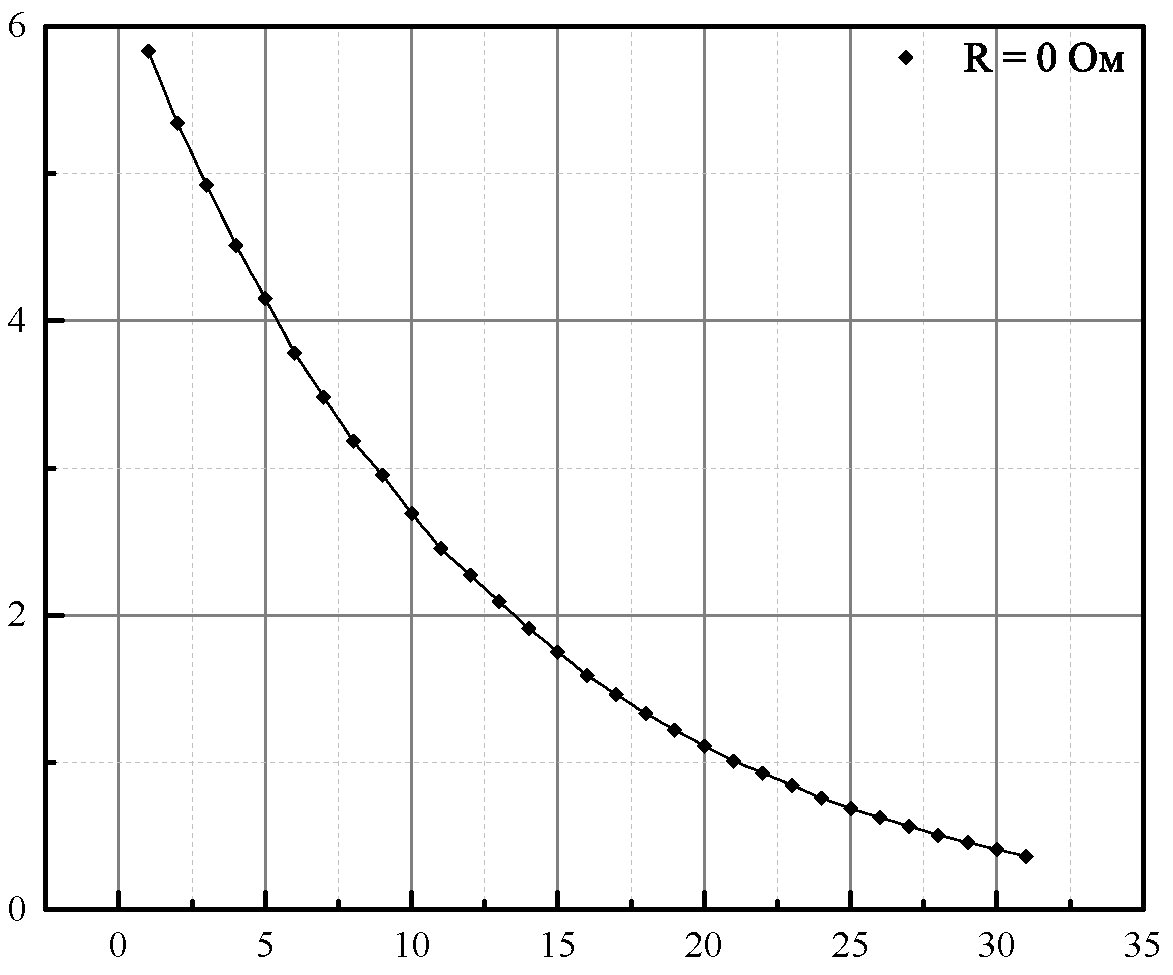
\includegraphics[width = 0.85\textwidth]{graph_2}
		\caption{графики зависимости перепада давления от расстояния до начала трубки}
		\label{fig:graph_2}
	\end{center}
\end{figure}

\section{Заключение}

\begin{enumerate}
	\item При выполнении данной работы были исследованы различные режимы течения газа по трубкам. На практике получена экспериментальная зависимость разницы давления в различных точках трубки в зависимости от расхода воздуха, идущего через трубку.
	\item Исследовались условия перехода течения из одного режима (ламинарного) в другой (турбулентный).
	\item Полученные зависимости разницы давлений от расхода воздуха согласуются с существующей теорией, описывающей движение газов и жидкостей в различных режимах.
	\item Определено значение вязкости воздуха : $\eta_{\text{эксп}} = \left(1,9 \pm 0,6\right) \cdot 10^{-6}$ Па$\cdot$с, при табличном значении $\eta_{\text{табл}} = \left(1,3 \pm 0,2\right) \cdot 10^{-6}$ Па$\cdot$с. Полученные значения равны в пределах погрешности.
	\item Основной вклад в погрешность итогового значения вязкости внесла погрешность измерения времени, а так же погрешности измерения давлений. Погрешности, связанные с установкой (погрешность линейных размеров установки, диаметра трубок) внесли меньший вклад в итоговое значение погрешности.
	\item Частично подтверждена теоретическая линейная зависимость падания давления с изменением расстояния от края трубки.
	\item Подтверждена формула Пуазейля для расхода газа при прохождении через трубку.
\end{enumerate}
\end{document}